%!TEX root=thesis.tex

\chapter{Radio Cross-identification}
\label{cha:passive-learning}
  % In this chapter I'll talk about a machine learning approach to the cross-identification problem (i.e. my pipeline).

  In this chapter, I develop a machine learning approach to the radio cross-identification problem. First, I will discuss different ways to train and use a classifier for the task, in particular framing the cross-identification problem as an object localisation problem. Then, I will discuss the available training data and how I chose to process it. Finally, I will present results against a dataset of expert labels, and compare these results to those found by other methods.

\section{Formalism}
\label{sec:cross-identification-formalism}
  
  \todo{Rewrite below into this section.}

  \todo{Explain why we're ignoring the radio part of this problem.}

  \subsection{Cross-identification as Object Localisation}
  \label{sec:object-localisation}

  \subsection{The Galaxy Classification Task}
  \label{sec:galaxy-classification-task}

% \section{Cross-identification as Binary Classification}
% \label{sec:framing-as-classification}
  
  When we look at the sky with radio telescopes, we see the radio emissions from
  the jets of AGNs. \todo{Add backlink.} Given an image of these radio
  emissions, we want to locate the host galaxy containing the associated AGN. In
  general, there may be multiple hosts associated with one radio object (such as
  in Figure \ref{fig:two-hosts}), but we make the assumption that there is only
  one. This is the same assumption made by Radio Galaxy Zoo \todo{cite:rgz-
  analysis-github(?)} and greatly simplifies the problem.

  \begin{figure}[!ht]
    \centering
    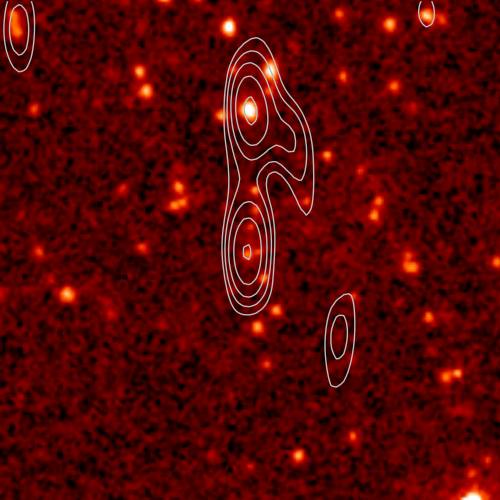
\includegraphics[width=0.5\textwidth]{images/CI0370C1_heatmap+contours.png}
    \caption{A radio object (ARG0003ra1) with two host galaxies. This radio
      object is actually two radio objects that have been incorrectly detected
      as one, and there is one host galaxy for each object.}
    \label{fig:two-hosts}
  \end{figure}

  We can interpret cross-identification as an object localisation problem. As
  input, we have an image of the radio sky, and we want to locate a host galaxy
  in this image. A common way to find an object in an image is by using a
  sliding window. A fixed-size image patch centred on each pixel is taken as a
  feature representation of that pixel. This is then used as input to a
  classification model which outputs a probability for each pixel, with higher
  probabilities corresponding to higher likelihood of the object being located
  at that pixel. The pixel with the highest rating is considered the location
  of the object. This approach can be improved by intelligently selecting
  candidate pixels and only testing these. For the cross-identification
  problem, we can use galaxy locations as candidate pixels, with galaxies found
  in infrared surveys such as WISE and SWIRE. Additionally, astronomical
  measurements such as flux are included in these surveys and these may be
  taken as additional features for each candidate pixel, giving more
  information to the classifier.

  This approach can be formalised as follows. Consider a set $\mathcal X$ of
  candidate host galaxies, and a radio object $r$ that we want to assign a
  host galaxy. Let $y : \mathcal X \to \{0, 1\}$ represent whether a given $x
  \in \mathcal X$ is the host galaxy associated with $r$. Under the assumption
  that a radio object has exactly one associated host galaxy, then there exists
  exactly one $x \in \mathcal X$ such that $y(x) = 1$, and for all other $x \in
  \mathcal X$, $y(x) = 0$. The cross-identification task then amounts to
  modelling $p(y(x) = 1 \mid x, r)$. Once this distribution is modelled, the
  host galaxy associated with $r$ is given by
  \begin{equation}
      \label{eq:cross-identification}
      \mbox{host}(r) = \underset{x}{\mbox{argmax}}\ p(y(x) = 1 \mid x, r).
  \end{equation}

  Ideally, $\mathcal X$ is the set of all galaxies. This is clearly
  intractable, so as an approximation we use a catalogue of infrared objects
  near the radio object of interest, taken from an infrared survey. We also
  make the assumption that the host galaxy is within $1'$ of the radio object
  --- while this doesn't hold in general, systems larger than $1'$ are rare and
  require human insight to discover \citep{banfield16}.

% \section{Data Sources}
% \label{sec:data}

%   To learn the cross-identification distribution (Equation \ref{eq:cross-identification}), we need a set of radio objects, a set of candidate host galaxies, and a set of existing cross-identifications for training. I have chosen to use the ATLAS radio survey for radio objects and the WISE survey for candidate host galaxies. The training cross-identifications are based on the Radio Galaxy Zoo.

%   \subsection{Radio Data}
%   \label{ssec:radio-data}

%     The ATLAS survey \citep{franzen15} \todo{talk about this in the astro chapter} provides both a catalogue of detected radio objects and a radio image of the CDFS and ELAIS-S1 fields.

%     The catalogue contains around 2400 objects in the CDFS field, all of which have been labelled by expert astronomers \citep{norris06}, by prior algorithms for automated cross-identification \citep{fan15}, and by Radio Galaxy Zoo volunteers \citep{banfield15}. The ELAIS-S1 field does not have Radio Galaxy Zoo classifications as it was not included by the Radio Galaxy Zoo researchers. The existence of expert, algorithmic, and crowdsourced labels makes ATLAS-CDFS an excellent set of radio objects for developing and testing machine learning approaches to cross-identification. Additionally, ATLAS is considered a pilot for the upcoming Evolutionary Map of the Universe survey, which will provide the majority of radio objects needing cross-identification in the future \citep{banfield15}.

%     \todo{talk about ATLAS image in the astro chapter}

%     The catalogue contains the name and position of each radio object, as well as various metadata such as the noise level and the flux. I have chosen to ignore the metadata and only use the position information. The positions are used to extract a $5' \times 5'$ from the full ATLAS image of the CDFS field, centred on each radio object. These image patches represent the radio object in the object localisation problem.

%   \subsection{Infrared Data}

%     Both the SWIRE and WISE surveys have imaged the CDFS field in infrared wavelengths. Of these, WISE is more commonly used, so I have chosen to use WISE as a source of candidate host galaxies. Like ATLAS, WISE provides both a catalogue of detected objects as well as images.

%     The WISE catalogue contains names, positions, and astronomical measurements for all detected infrared objects. I used the positions to generate features for each candidate host, and the raw flux measurements as additional features. Feature generation is described in Section \ref{sec:features}. I chose to use the fluxes as they have the most physical meaning \todo{citation needed}.

%     I have chosen to not use image data from WISE. Preliminary experiments showed that there was not much information gained from the use of infrared images, and using infrared images made the classifier more complex. Future work may use infrared images to improve the classifier.

%   \subsection{Radio Galaxy Zoo Consensus Labels}
%   \label{sec:consensuses}

%     \todo{move lots of this to the astro section}
    
%     Radio Galaxy Zoo volunteers are first asked to select combinations of radio
%     objects that correspond to one radio source, and are then asked to select
%     the location of the corresponding host galaxy \citep{banfield15}. Each
%     radio subject is labelled by multiple volunteers. These labels are then
%     collated as follows. First, the most common combination of radio objects is
%     selected, and all labels that have a different combination are discarded.
%     This radio combination is called the consensus radio combination. Then, the
%     density of host location labels is estimated using Gaussian kernel density
%     estimation (KDE), and the highest density location is selected. This is
%     called the consensus host location. The consensus host location is then
%     matched to the nearest infrared object.

%     An alternative way to find the consensus host location is by using a
%     clustering algorithm such as $k$-means. Host locations are clustered and
%     the cluster containing the most locations is taken to represent the
%     consensus; the consensus location is then the mean of the cluster. This is
%     faster and more robust than using KDE, but requires $k$ to be known. $k$
%     can be estimated using an algorithm such as PG-means \citep{hamerly07} or by
%     choosing $k$ to minimise some information criterion \todo{cite:sklearn}.
%     The consensus labels for the data associated with this thesis were found in
%     this way, fitting a Gaussian mixture model to the host locations with the
%     number of Gaussians chosen to minimise the Bayesian information criterion.

%     Repeated volunteer labelling helps to reduce noise in the labels. This is
%     necessary as the volunteers are not experts, and may incorrectly label the
%     subject. The hope is that the majority of volunteers will correctly label
%     subjects, which seems to be the case for radio subjects where more than
%     75\% of volunteers agree \citep{banfield15}. The number of times a radio
%     subject is shown to different volunteers is called the redundancy. The
%     redundancy is 5 if the subject is a compact source, and 20 for all other
%     sources. These numbers were chosen based on the redundancy levels of the
%     original Galaxy Zoo project [Banfield, personal communication] \todo{Is
%     this how to cite personal communication? Alternatively, is this written
%     down somewhere?}. Since labels with radio combinations that disagree with
%     the consensus are discarded, the redundancy is usually lower in practice
%     when finding the host location. This can lead to very low redundancy input
%     to KDE, causing KDE to fail. This failure can usually be caught, but the
%     existing solution in this case is to take the mean of all host locations.
%     This is not the consensus host location in general. Another effect is that
%     since more complex sources have higher levels of disagreement in the radio
%     combination stage, more complex sources have more discarded volunteer
%     labels, and thus lower redundancy --- so more complex sources have more
%     noise in their labels.

%     The training data are generated by assigning each infrared object a binary label: $0$ if the object is not associated with a radio object, and $1$ if the object is associated with a radio object.

%   \subsection{Norris Labels}
%   \label{sec:norris}

\section{Feature Selection}
\label{sec:features}

  To train a machine learning method to solve the galaxy classification task,
  we must find a representation of galaxies in a feature space $\mathbb{R}^D$.
  In this section we describe and motivate our choice of galaxy features,
  extracted from both infrared and radio surveys.

  \subsection{Infrared Features}
  \label{sec:ir-features}

    The WISE catalogue (Section \ref{sec:wise}) contains magnitude information
    for each object. There are four such magnitudes --- $w1$, $w2$, $w3$, and $w4$ ---
    each representing the amount of light emitted by the object in a different
    range of wavelengths.

    We chose to use all four magnitudes as features. Since the features are
    magnitudes, they are on a logarithmic scale, and we found that in practice
    classification performance improved when the magnitudes were converted to
    fluxes. We performed this conversion with the formula
    \[
      f = 10^{-0.4m}
    \]
    where $f$ is the flux and $m$ is the magnitude. This is the inverse of Equation \ref{eq:apparent-magnitude}, and gives the flux in arbitrary, but linear, units.

    \begin{figure}[!ht]
      \centering
      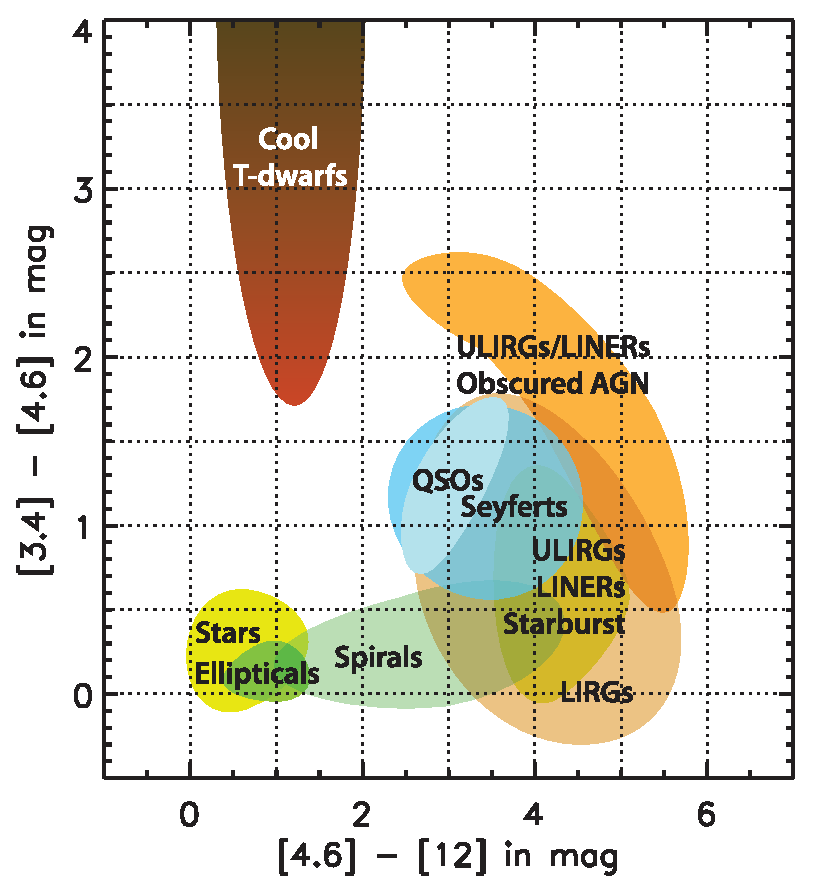
\includegraphics[width=0.5\textwidth]{images/wise_colour-colour}
      \caption{WISE colour-colour diagram showing the colours of various
        astronomical objects. The horizontal axis is $w2 - w3$ and the vertical
        axis is $w1 - w2$. Reproduced from \citep{wright10}.}
      \label{fig:wise-colour-colour}
    \end{figure}

    The ratios between infrared fluxes are indicators of physical galactic
    properties such as star formation and dust \todo{Find a source on this ---
    Probably the WISE paper wright10}. In practice, the $w1 - w2$ and $w2 - w3$
    ratios are most commonly used (such as in Figure \ref{fig:wise-colour-
    colour}), so we chose to use these ratios as features. Once again, we used
    a linear scale, computing the ratios using equation \ref{eq:magnitude-
    difference}.

    Also available were the unprocessed infrared images captured in the survey.
    Under the assumption that the large scale infrared structure of a galaxy is
    unchanged by an AGN, we chose to ignore the images themselves and focus on
    features obtained from the catalogue. This greatly simplified feature
    selection with minimal expected impact on the classification performance.
    Future work may investigate the effectiveness of features extracted from
    infrared images on classification performance, but this is out of the scope
    of this thesis.

    \todo{Discuss SWIRE features.}

    % The SWIRE catalogue (Section \ref{sec:swire}) also contains colour information for each contained object, but only fluxes rather than magnitudes. \todo{Read the SWIRE colour-colour diagram and continue this.}

    % Both WISE and SWIRE catalogues contain the positions of each object. The distance from each object to the centre of the closest radio object is used as a feature representing that object. This noticeably improves classification performance \todo{make an experiment showing this, and probably also showing that the other features are good}.

  \subsection{Radio Features}
  \label{sec:image-features}

    While the infrared catalogues include measurements on individual galaxies,
    the ATLAS radio catalogue does not. This is because galaxies are not
    visible in radio, so while galaxies are directly represented in an infrared
    catalogue they are not in a radio catalogue. Galactic features must thus be
    extracted from the radio images directly. We chose to use a convolutional
    neural network, as described in Section \ref{sec:image-features}.

    \subsubsection{Building a Model for Feature Extraction}
    \label{sec:feature-extraction-model}

      We chose to use a convolutional neural network (CNN) with two
      convolutional and max pooling layers, shown in Figure \ref{fig:radio-
      cnn}. This resulted in an 800-dimensional feature vector. For training
      this network, we added a 64-dimensional dense layer mapping to a
      1-dimensional output, and trained the entire network to match the
      consensus Radio Galaxy Zoo labels.

      \begin{figure}[!ht]
         \centering
         % \usepackage[usenames,dvipsnames]{pstricks}
% \usepackage{epsfig}
% \usepackage{pst-grad} % For gradients
% \usepackage{pst-plot} % For axes
% User Packages:
% 
% 
\psscalebox{0.6 0.6} % Change this value to rescale the drawing.
{
\begin{pspicture}(0,-2.5333333)(20.966753,2.5333333)
\psframe[linecolor=black, linewidth=0.04, fillstyle=solid, dimen=outer](6.623895,1.8666667)(4.5667524,-0.1904762)
\psframe[linecolor=black, linewidth=0.04, fillstyle=solid, dimen=outer](7.1381807,1.352381)(5.081038,-0.7047619)
\psframe[linecolor=black, linewidth=0.04, fillstyle=solid, dimen=outer](7.652467,0.83809525)(5.5953236,-1.2190477)
\psframe[linecolor=black, linewidth=0.04, fillstyle=solid, dimen=outer](8.166752,0.32380953)(6.1096096,-1.7333333)
\psframe[linecolor=black, linewidth=0.04, fillstyle=solid, dimen=outer](11.242077,1.4666667)(9.766752,-0.008658009)
\psframe[linecolor=black, linewidth=0.04, fillstyle=solid, dimen=outer](11.6109085,1.0978355)(10.135584,-0.37748918)
\psframe[linecolor=black, linewidth=0.04, fillstyle=solid, dimen=outer](11.979739,0.7290043)(10.504415,-0.74632037)
\psframe[linecolor=black, linewidth=0.04, fillstyle=solid, dimen=outer](12.348571,0.36017317)(10.873246,-1.1151515)
\psframe[linecolor=black, linewidth=0.04, fillstyle=solid, dimen=outer](15.184934,1.0666667)(14.166752,0.048484847)
\psframe[linecolor=black, linewidth=0.04, fillstyle=solid, dimen=outer](15.43948,0.8121212)(14.421298,-0.2060606)
\psframe[linecolor=black, linewidth=0.04, fillstyle=solid, dimen=outer](15.694025,0.55757576)(14.675843,-0.46060607)
\psframe[linecolor=black, linewidth=0.04, fillstyle=solid, dimen=outer](15.94857,0.3030303)(14.930388,-0.7151515)
\psframe[linecolor=black, linewidth=0.04, fillstyle=solid, dimen=outer](18.203115,0.6666667)(17.766752,0.23030303)
\psframe[linecolor=black, linewidth=0.04, fillstyle=solid, dimen=outer](18.312206,0.55757576)(17.875843,0.121212125)
\psframe[linecolor=black, linewidth=0.04, fillstyle=solid, dimen=outer](18.421297,0.44848484)(17.984934,0.012121212)
\psframe[linecolor=black, linewidth=0.04, fillstyle=solid, dimen=outer](18.530388,0.33939394)(18.094025,-0.096969694)
\rput[bl](5.7667522,2.2666667){$32 \times 71 \times 71$}
\rput[bl](10.166752,2.2666667){$32 \times 14 \times 14$}
\rput[bl](14.166752,2.2666667){$32 \times 5 \times 5$}
\rput[bl](17.366753,2.2666667){$32 \times 1 \times 1$}
\psframe[linecolor=black, linewidth=0.04, dimen=outer](20.966753,1.0666667)(20.566751,-0.53333336)
\rput[bl](20.566751,2.2666667){$32$}
\psframe[linecolor=black, linewidth=0.02, fillstyle=solid, dimen=outer](8.051859,-0.8992908)(7.511433,-1.4397163)
\psframe[linecolor=black, linewidth=0.02, fillstyle=solid, dimen=outer](12.251859,0.10070922)(11.911433,-0.2397163)
\psframe[linecolor=black, linewidth=0.02, fillstyle=solid, dimen=outer](15.851859,-0.39929077)(15.711433,-0.5397163)
\psframe[linecolor=black, linewidth=0.02, fillstyle=solid, dimen=outer](12.151858,-0.69929075)(12.011434,-0.8397163)
\psframe[linecolor=black, linewidth=0.02, fillstyle=solid, dimen=outer](15.751859,0.0)(15.711433,-0.03971631)
\psframe[linecolor=black, linewidth=0.02, fillstyle=solid, dimen=outer](18.451859,0.10070922)(18.411432,0.060283687)
\psline[linecolor=black, linewidth=0.02](8.03614,-0.9071925)(12.03614,-0.7210884)
\psline[linecolor=black, linewidth=0.02](8.031646,-1.4239547)(12.040634,-0.825193)
\psline[linecolor=black, linewidth=0.02](12.23614,0.08831308)(15.7352915,-0.0063670413)
\psline[linecolor=black, linewidth=0.02](12.231646,-0.22844914)(15.726303,-0.028838951)
\psline[linecolor=black, linewidth=0.02](15.847376,-0.40831614)(18.434168,0.099250935)
\psline[linecolor=black, linewidth=0.02](15.847376,-0.5363143)(18.416191,0.06779026)
\psline[linecolor=black, linewidth=0.02](18.508915,0.31476077)(20.611092,1.0454048)
\psline[linecolor=black, linewidth=0.02](18.478146,-0.09016045)(20.58542,-0.5091328)
\psframe[linecolor=black, linewidth=0.04, fillstyle=solid, dimen=outer](2.6443307,1.3167521)(0.0,-1.3275784)
\rput[bl](0.8500857,2.2833333){$80 \times 80$}
\psframe[linecolor=black, linewidth=0.02, fillstyle=solid, dimen=outer](2.4299755,0.9778653)(1.7352916,0.28318152)
\psline[linecolor=black, linewidth=0.02](2.3764367,0.9770822)(7.6681905,0.008276656)
\psline[linecolor=black, linewidth=0.02](2.3706596,0.28333333)(7.6906343,-0.29167688)
\psframe[linecolor=black, linewidth=0.02, fillstyle=solid, dimen=outer](7.9685254,0.034042552)(7.6281,-0.30638298)
\rput[bl](12.000086,-2.4833333){$10 \times 10$
 convolution}
\rput[bl](16.050085,-2.5333333){$5 \times 5$
  max pooling}
\rput[bl](2.8000855,-2.4833333){$10 \times 10$
 convolution}
\rput[bl](8.050086,-2.5333333){$5 \times 5$
  max pooling}
\end{pspicture}
}


         \caption{Convolutional neural network for radio feature extraction.}
         \label{fig:radio-cnn}
       \end{figure}

       This introduced a degree of peeking, as the network was effectively trained on the galaxy classification task. This is mitigated in two ways: Firstly, there are many more degrees of freedom in the dense layer as in the classifier we used later, so the CNN could at best partially learn the classification task in the short time it was trained for. Secondly, the dense layer was not included in the final feature extractor, and the CNN was not fine-tuned --- features output by the CNN were fixed as inputs to the classifier. A better approach would be to use a convolutional autoencoder, which would eliminate the peeking entirely and allow training on radio data with no labels at all, but this was computationally infeasible for this project.

    \subsubsection{Filters}
    \label{sec:image-filters}

      

\section{Choosing a Binary Classifier}
\label{sec:binary-classifiers}
  
  \begin{figure}[!ht]
    \centering
    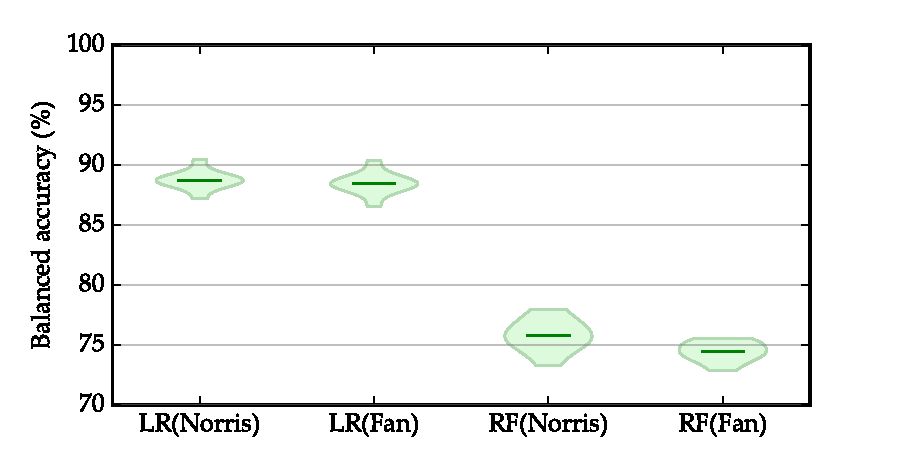
\includegraphics[width=\textwidth]{images/experiments/lr_rf}
    \caption{Comparison of logistic regression and random forests on the galaxy classification task, trained on the \citet{norris06} and \citet{fan15} label sets, and tested against the \citet{norris06} label set.}
  \end{figure}

  To compare the performance of logistic regression with random forests on the galaxy classification task, I performed the following experiment. First, I generated five test sets of WISE objects. Then, using all other WISE objects as a training set, I trained a logistic regression classifier for each test set, first using labels from \citet{norris06}, and then, separately, using labels from \citet{fan15}. I then computed the balanced accuracy for each classifier. Finally, I repeated the experiment for random forests.

  To generate the test sets, I first selected at random half of all ATLAS objects. I then added all WISE objects within $1'$ of a selected ATLAS object to the test set. This was repeated for each test set. The motivation for first selecting ATLAS objects rather than drawing WISE objects directly is that WISE objects have overlapping features since radio features are taken from a patch of sky centred on each object, and WISE objects tend to be close together. Objects from the test sets were then removed at random until all test sets were the same size. Each test set contained $13605$ WISE objects.

\section{Handling Crowd Labels}
\label{sec:rgz-crowd-labels}

  While we want to train a classifier on the crowdsourced labels from the Radio Galaxy Zoo, it is unclear how we should aggregate the labels. Some methods for aggregation are described in Section \ref{sec:crowd-labels}. Which method will perform best on a dataset is dependent on the dataset itself, so we tested both variants of the \citeauthor{raykar10} algorithm and majority vote on the galaxy classification task.

  \todo{Compare majority vote and Raykar.}

\section{Results}
\label{sec:rgz-results}
  
  \subsection{Classifying Galaxies}

    \todo{Make this writing considerably less terrible.}

    The infrared objects were partitioned into a testing set and a training set as follows. First, the radio objects were partitioned into a radio testing set and a radio training set, with the radio testing set containing $452$ objects and the radio training set containing $1811$ objects. Infrared objects were then added to the infrared testing set if they were within $1'$ of a radio object in the radio testing set, and added to the infrared training set otherwise. This was done because infrared objects that were close together had overlapping radio features, and thus random partitioning would result in the training set containing many of the features found in the testing set. The partitioning resulted in $5922$ objects in the testing set and $18218$ objects in the training set.

    For each infrared object, features and labels were generated as described in Sections \ref{sec:features} and \ref{sec:consensuses}, respectively. Note that the labels were sourced from the Radio Galaxy Zoo. A logistic regression classifier was then trained on the training set using binary cross-entropy loss, with loss of each data point weighted based on the frequency of its label.

    The classifier was then used to classify the objects in the testing set. The labels were compared to those found by \citet{norris06} as described in Section \ref{sec:norris}, resulting in $80.14\%$ balanced accuracy.
    \todo{This number is out of date.}

    \todo{ROC/precision--recall curves}

    \begin{figure}[!ht]
      \centering
      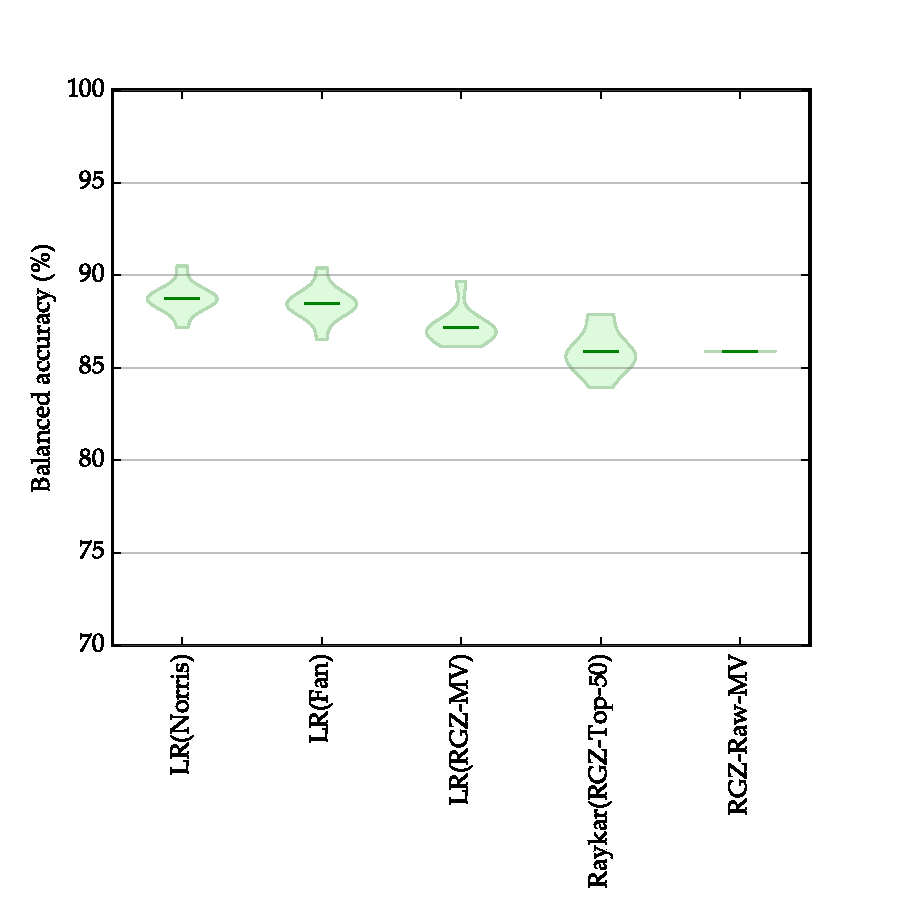
\includegraphics[width=\textwidth]{images/experiments/predictors.pdf}
      \caption{Performance of logistic regression on the galaxy classification task, trained on different sets of labels and tested on the galaxies where \citeauthor{norris06} and \citeauthor{fan15} labels agree. LR($Y$) indicates logistic regression trained on $Y$. RGZ-MV is the set of majority vote labels from the Radio Galaxy Zoo. RGZ-Raw-MV is the majority vote of all crowd labels and is included for comparison.}
    \end{figure}

  \subsection{Number of Training Examples}

    \begin{figure}[!ht]
      \centering
      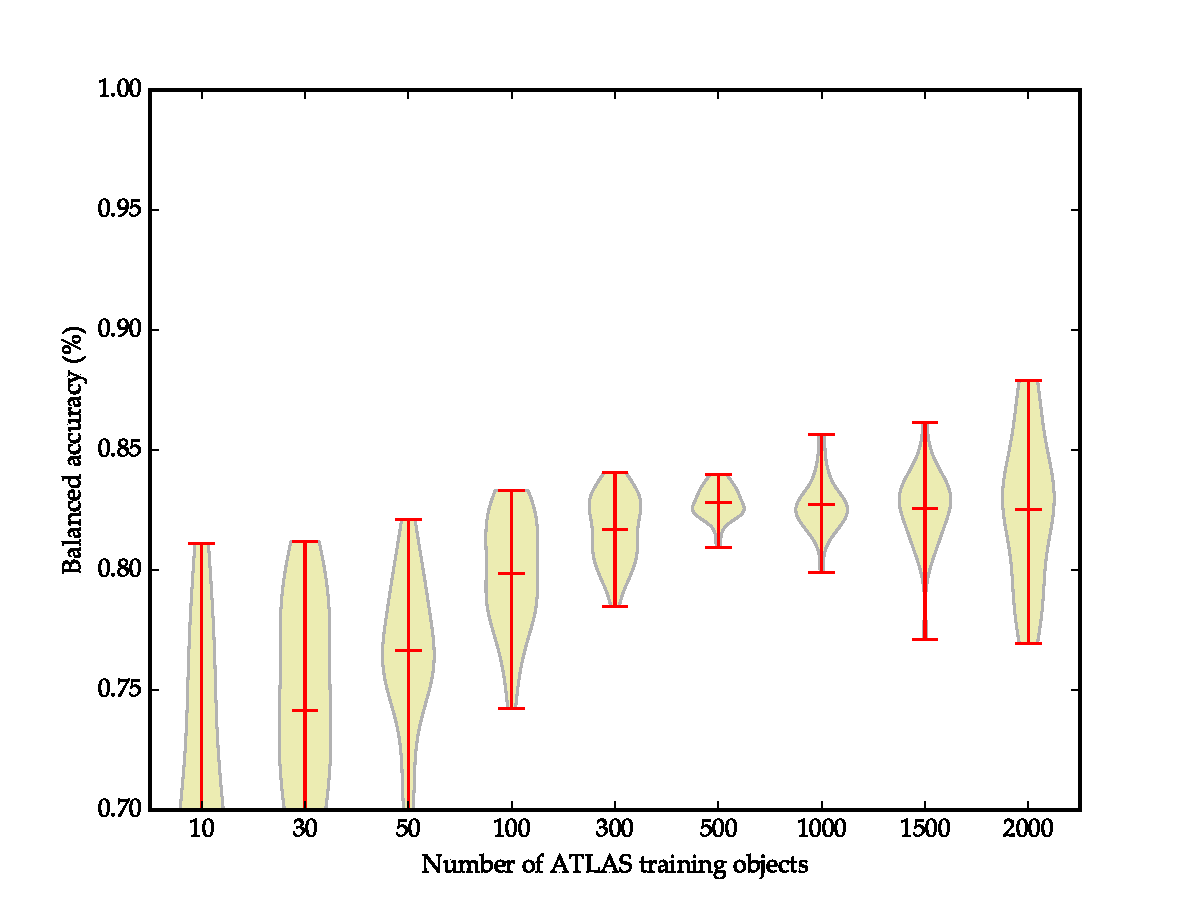
\includegraphics[width=\textwidth]{images/experiments/passive.pdf}
      \caption{Performance of logistic regression on the galaxy classification task, trained on different amounts of the \citeauthor{norris06} label set.}
    \end{figure}

\section{Discussion}
\label{sec:rgz-discussion}